
\documentclass[10pt]{article}
\usepackage[margin=1in]{geometry}
\usepackage{amsmath}
\usepackage{amssymb}
\usepackage{setspace}
\usepackage{graphicx}
\usepackage{caption}
\usepackage{listings}
\usepackage{enumitem}
\usepackage{subfigure}


\begin{document}

\title{ECE 4750 Lab 4: Ring Network}
\author{Avinash Navada (abn44) \& Akshay Dongaonkar (akd54) 
		\& Vivek Gaddam (vrg22)}
\maketitle


\section{Introduction}

With processors hitting the power wall and Moore's Law not the primary vehicle
in increasing general computing performance, designers have chosen to
replicate processing units on a single chip. 
This process is called parallelism. 
The idea is that multiple compute units can do different work at the same time
to increase performance.
However, when multiple compute units need to communicate, they need a network
to pass their messages. \par

Given that many tasks are not easily made parallel, there is message overhead.
This leads to designers needing to develop a fast and reliable
on chip interconnect network.
In this lab, we explore the performance of a ring topology under multiple
routing algorithms. \par

In the project management section, we will lay out our project roadmap,
distribution of work, and member roles.
In the baseline design section, we will describe our ring topology and our 
greedy oblivious routing algorithm.
In the alternative design section, we will describe an adaptive routing 
algorithm to increase performance under adversarial traffic patterns.
This routing algorithm ingests greater information on the congestion within
the network to route intelligently.
In the evaluation section, we compare the performance under both routing
algorithms and the performance of the topology in general. 
We found that generally the adaptive scheme is not more effective to the 
oblivious, baseline scheme in throughput and zero load latency. 
One can always construct a specific scheme to defeat a routing algorithm that
does not have perfect global state; thus we say generally pareto-optimal.


\section{Project Management}

We assigned Akshay to be the architect,
Avinash to be the verification lead,
and Vivek to be the design lead.
Our initial project roadmap was rather aggressive and required us to be 
finished by Sunday, November 9\textsuperscript{th}, since we planned on 
trying out an extension or two for this lab. 
Our expected and actual work patterns are shown in Figure~\ref{fig:gantt}.
Clearly, we still have not gotten the hang of working under a predictable
and incremental schedule pattern.
We aim to fix this for the final lab.
It is our last chance to do so, and we are highly motivated in this goal.
 \par

The work was divided as follows:
Vivek worked on most of the baseline RTL code.
Akshay worked exclusively on the writeup and the evaluations of the designs.
Avinash finished the baseline design and implemented the alternative design.
He also completed our testing suite.
Akshay's work was lacking in this lab; he was sick most of the first week
and part of the second week of this lab. \par

The work was approached by simultaneously starting the baseline 
implementation and testing, followed by the lab writeup shortly after.
Baseline paths that were completed were promptly tested. 
As soon as the baseline implementation was complete and successfully tested, 
Avinash moved on to the alternative design implementation and testing 
(which included adding additional test cases for the alternative design). 
Each team member helped others debug as much as they could. 
Due to Akshay being sick and Vivek having a tough workload in other classes,
we were unable to implement an extension. 
We are sad that we were unable to complete an extension even at the advanced
stage of this semester. 


\section{Baseline Design}

The baseline design for our lab network has 8 nodes in a ring configuration
for its topology. 
Each node contains a message producer/consumer (also known as Input/Output 
terminals), a router that the terminal connects to,
and two outgoing channels from the router to other routers in the ring.
This topology is logically shown in Figure 2. 
Each router connects to two other routers; the west channel of router $n$ 
is the channel connecting to router $n-1$ and 
the east channel of router $n$ connecting to router $n+1$.
This arithmetic is done under modulo 8.
With this topology, it is easy to see that there is a path from every terminal
to every other terminal.
The path is as follows:
\begin{enumerate}[nolistsep]
	\item Take the path to your router
	\item Go east until you get to the router number that corresponds to your 
		  destination address
	\item Take the path leading to the terminal
\end{enumerate}
Naturally, this is not the minimal path in the network; we simply want to show
how our network of terminals is connected.
This property is highly desirable as we need to communicate with 
all of our components! \par

The messages that our network transmit have a parameterized structure.
There is a payload size, a source/destination tag size determined by the number
of addresses (in our case eight), and an opaque bit size.
These messages are ingested at port 1 of our router at a given node, and based
on a routing algorithm, are directed to either ports 0-2.
Regardless of the routing algorithm, port 1 is chosen if and only if 
the source and destination addresses are the same.
Depending on the routing algorithm, either port 0 or 2 is chosen for other
cases of source and destination addresses. \par

The physical datapath on which the messages travel on is shown in Figure 3.
Each router port is buffered by an input queue of size four which carries
network messages. 
Under some control logic soon to be discussed, an encoding of the 
\texttt{xbar\_sel*} bits allows one message meant for one output port to
traverse the crossbar at every cycle.
This allows up to three discrete messages to traverse the router on any 
given cycle.
A val/rdy interface mediates transfer of the packet out of the router. 
This process repeats as long as there are packets in the input queues.
The box shown in Figure 3 around our router datapath is the interface for our 
Router Base module. 
We repeat this modular design in our control logic.
The control logic is stored separately in another module so as to follow the
design pattern of the control-datapath split. 
The reason we did this is because it made it easier to implement our 
alternative design.
We did not need to change much of our baseline datapath to implement an 
entirely new algorithm relying pseudo-global network information. \par

The control logic consists of multiple modules to route network packets.
This design was to make it easier to implement multiple routing algorithms
and to decouple the task of ingesting a packet, determining its destination,
and actually sending the message to the correct port. \par
The Router Input Terminal Control module implements the logic to ingest packets into
a router. 
If a packet is from the input terminal, the module performs deadlock avoidance 
checks by ensuring there is a bubble in our network so that packets can still
route freely.
A bubble is simply a free queue slot in which new packets reside.
The route computation module then comes into play to route the packet.
If a packet originates from the network, it checks whether it needs to accept
that packet for its terminal or keep routing. 
If the router needs to accept the packet for its terminal, it sends the
corresponding signal to the Router Output Control unit that a packet needs to 
be placed on the port 1 queue. 
If the router needs to keep routing, it will send the corresponding signal to
the Router Output Control unit that a packet needs to be placed on the port 0
queue if it needs to continue traveling westward or the port 1 queue if it 
still needs to continue traveling eastwards.
Packets entering the router via the port 1 (west) or port 2 (east) input queues
are directed along the same path (a west-bound packet continues west by routing through
the router's east output terminal) by a Router Input Control Module (not to be 
confused with the Router Input Terminal Control Module, which deals with packets
 in the router's terminal queue and performs route computation). If the current 
 router is the destination of the packet, the Router Input Control Module requests
 the Router Output Control unit to place the packet on the port 1 input queue.  \par

Since there is contention on each of the three output ports, the 
Router Output Control module mediates access to the ports. 
The vehicle for access to ports is a round-robin arbiter. 
Given multiple packets that need to travel out of a singular port, the arbiter
allows only one packet to traverse the crossbar to continue routing. 
This flow control scheme is entirely given by the arbiter module provided. \par

As mentioned previously, the final module (Route Computation) actually provides
the routing logic required to move packets across the network.
In the baseline implementation, we implemented a greedy algorithm.
We routed packets east if the router hop count to the destination was less than
the router hop count to the west. 
%Of course, in the situation where the source address was equivalent to the 
%destination address, we routed the packet back into the terminal without
%letting the packet interact with another router. 
We were able to compute the router hop count because our network is static. 
This led to a simple and efficient route computation unit, which will be 
discussed further in our evaluation of our two designs.

\section{Alternative Design}

Our alternative design changes our route computation. 
Instead of simply greedily routing packets on the shorter router hop count
path, we look at the channel queues of the channel each router's packet 
takes up to 2 hops away. 
To clarify, we look at router $n-1$'s and $n-2$'s channel sizes 
for router $n$ as well as router $n+1$'s and $n+2$'s channel sizes.
This size is their congestion at their ports. 
Of course, this arithmetic for router names is done under modulo 8. 
Given this congestion factor, we determine whether we want to route packets 
through the path with the longer hop count. 
A representation of the new control signal is shown in Figure 5.\par

There are, however, special cases to consider. \\
As stated before, if the source and destination address are the same, then the
router immediately routes back to the input terminal for a router hop count 
of 1.
This is always the optimal routing path.
Another special case is for the destination one address away. 
This is equivalent to the two router hop case.
In this case, we always route greedily. 
This is because the maximum amount of time we would have to wait on a queue
would be 6 cycles: 
potentially 3 cycles for arbitration to allow the channel in the other 
direction to route to the output terminal port (port 1) and another three
cycles for your own channel to route to the output terminal port.
If there were loopback requests from the terminal, there could be up to 10 
packets attempting to enter a given terminal.
However, if the source was one channel away from the destination router and the
rest of the network was empty, it would still take 10 cycles to route the 
opposite direction. 
There would be 7 cycles of empty traffic and three cycles of pure waiting time.
Therefore, either way leads to 10 cycles of waiting.
It makes no sense to route the other way, \textit{ever}.
So, we will simply route greedily in that case. \par

In the other cases so far, we simply treat congestion as a one router hop 
cost.
So if a channel going east has a 2 queue length delay at the first router 
and the hop count is 4 to the destination, we say routing east has a cost of 7.
Vice versa, a channel going west having no delay and no congestion has a cost
of $ 0 + 4 =4 $. 
Therefore, we route west. 
We route on whichever route has a lower cost. \par

We simulate wire delay in queue size/length by pipelining the channel congestion
information from one and two hops over through a module that contains registers 
to relay our control unit. Two such ``congestion pipelines'' had to be implemented
in the alternative top-level ring module to accommodate for CW and CCW packet flow
directions.
This was a modification done in the datapath that was encapuslated in a 
module, 
This is fairly simple, however, as we are simply inducing wire delay. \par
This does lead to imperfect information though. We are not considering congestion 
information from 4 other channel queues that are further away, and pipelining the 
congestion information implies that we are receiving old information. This delay 
is one reason we chose to look at 2 hops over east and west instead of 4 (which 
would cover the whole network). 
However, we assume the network is close to steady state and that general 
congestion earlier implies general congestion later. 
This is some type of temporal prediction of network state. \par

As far as the design of the alternative network goes, we were able to plug in our
new routing algorithm without having catastrophic debugging issues. We could also 
have pipelined congestion information from neighboring router input queues instead 
of only looking at channel queues (which may have been a better indicator of actual
congestion in a given route). 

\section{Testing Strategy}

We began the testing process by developing directed tests for the baseline router 
components and verifying them on the functional model. These components were the 
Router Input Control, Router Input Terminal Control, and Router Output Control 
Units. We tested each of these components as soon as they were implemented. Next
we tested the baseline router itself and finally the entire baseline ring network
once they were implemented. This process was repeated for the alternative 
design; we re-used all the baseline tests but added some more tests to target the 
new adaptive routing algorithm. 

We tried to ensure that we were testing all possible use-case scenarios of the modules
we implemented. The Router Input Control module required simple testing since its
functionality is simple. The module only directs packet flow along the same 
direction in the network so we tested the three different possible scenarios: west-bound packet
continuing west, east-bound packet continuing east, packet bound to current router is 
directed to current router. For the Router Input Terminal Control, we tested 

\section{Evaluation}

Figure~\ref{fig:patterns} below is quite indicative of the performance of
our baseline and alternate implementations of a ring network.
There are multiple traffic patterns under consideration, such as uniform 
random, tornado, and rotation. 
In every single traffic pattern, the baseline implementation is pareto-optimal
to the alternative implementation. \par

In some cases, the throughput of the traffic patter almost drops by half.
This is in reference to Partition2 traffic, 
and to a lesser extent, Uniform Random. 
Such a big dropoff was not initially expected. 
Weren't we in fact increasing ideal throughput by distributing congestion in 
the network, allowing more packets to be in flight? 

Additionally, the zero-load latency drop off should not have been that drastic.
We were expecting results along the lines of tornado; maybe a very slight
increase in latency, but not on the order of multiples of cycles. 
This means that our adaptive routing algorithm is miscalculating the cost
of rerouting to the non greedy path. 
The cost needs to be higher in our non-greedy path to make sure that the path 
is taken only when it will reduce latency. \par

The problem is that we do not have global informatino about our network.
Compounding the problem is the staleness of the global information we have.
We are possibly delayed by four cycles in getting network state at some time
$t$. 
Now, this should not matter in our test programs because the network streams
are constant and elephant in nature. 
However, on any real workload, this strategy will surely falter as nodes 
are taking longer paths for no benefit. 

\newpage
\section {Tables and Diagrams}

% % Figure: Gantt Chart

\begin{figure}[h]
	\centering
	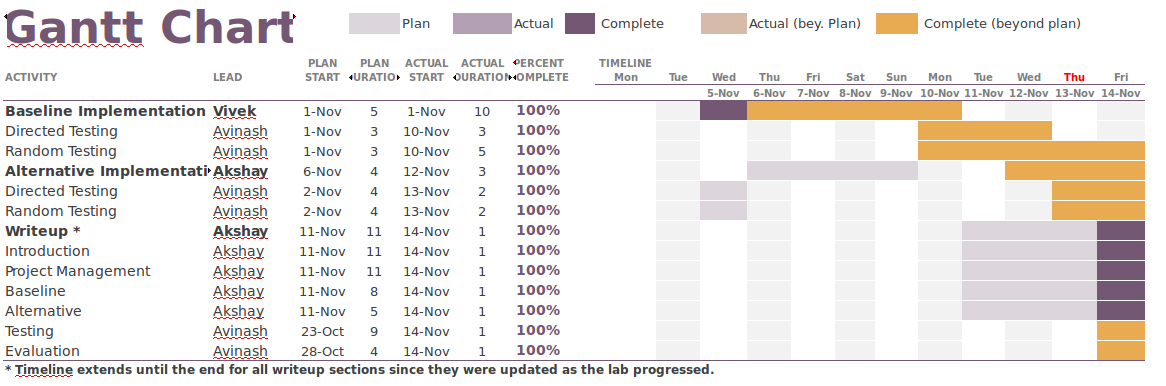
\includegraphics[scale=0.4, angle=90]{gantt}
	\caption{Gantt Chart.}
	\label{fig:gantt}
\end{figure}

\begin{figure}[h]
	\centering
	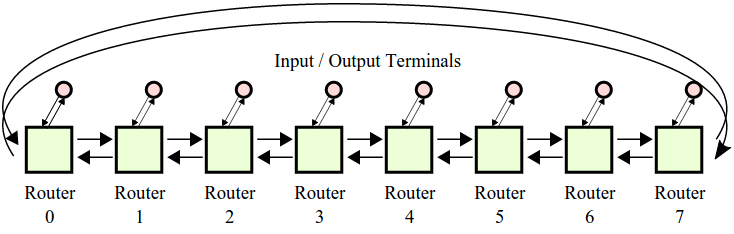
\includegraphics[scale=0.5]{topology}
	\label{fig:topo}
	\caption{Network Topology of our Ring}
\end{figure}

\begin{figure}[h]
	\centering
	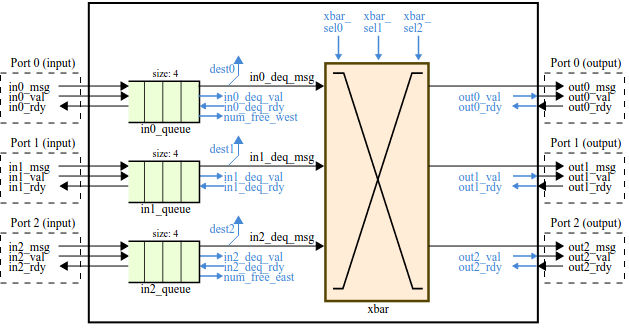
\includegraphics[scale=0.7]{dpath}
	\label{fig:dpath}
	\caption
	{
		The Datapath for our Router.
		Each channel mediates transmission via val/rdy interfaces.
		An arbiter allows messages to go in and out in a round robin fashion.
	}
\end{figure}

\begin{figure}[h]
	\centering
	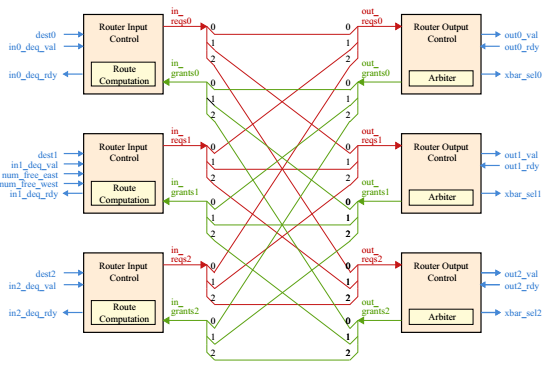
\includegraphics[scale=0.7]{baselinectrl}
	\label{fig:ctrl}
	\caption
	{
		The Control Unit for our Router.
		The Router Input Control module routes existing packets in our network 
		based on destination and accepts new packets to transfer.
		The Route Computation module determines on which port the packet will
		exit.
		The Router Output module allows packets to exit on a port by performing
		some arbitration. 
	}
\end{figure}

\begin{figure}[h]
	\centering
	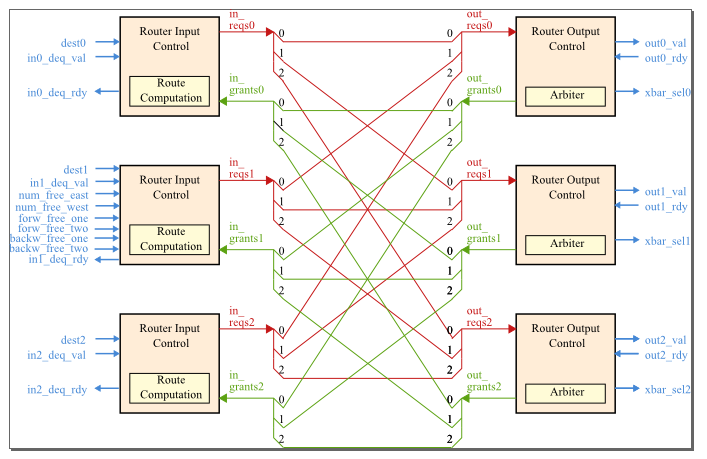
\includegraphics[scale=0.7]{altctrl}
	\caption{The Control Store for the Adaptive algorithm. 
			 Notice that the inputs now contain channel information as well.}
	\label{fig:altctrl}
\end{figure}

\begin{figure}[h]
\subfigure[Uniform Random]{
	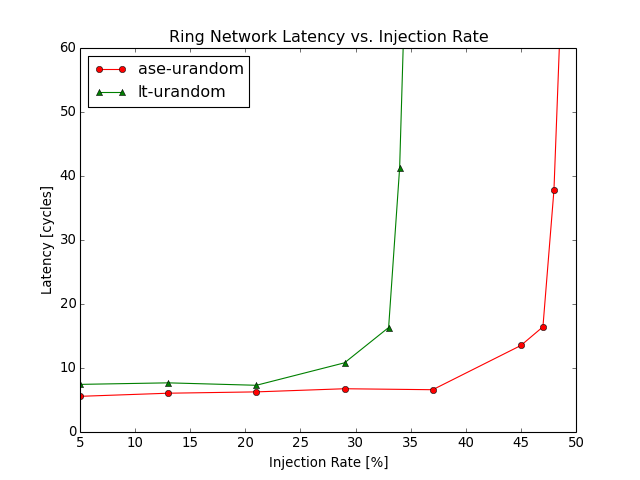
\includegraphics[width=0.33\textwidth]{lab4-net-urandom-plot}
}
\subfigure[Partition2]{
	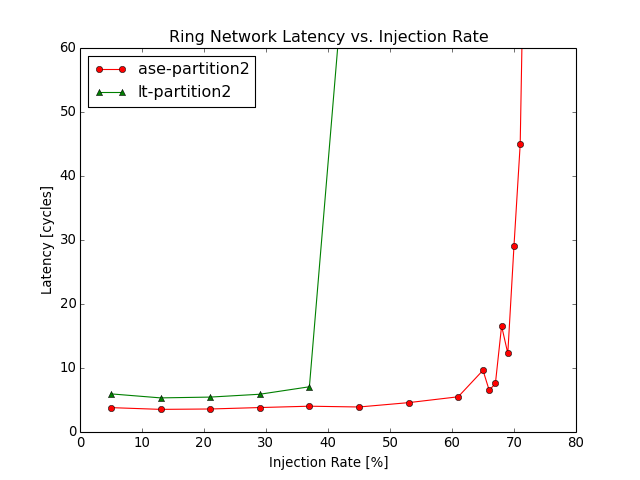
\includegraphics[width=0.33\textwidth]{lab4-net-partition2-plot}
}
\subfigure[Partition4]{
	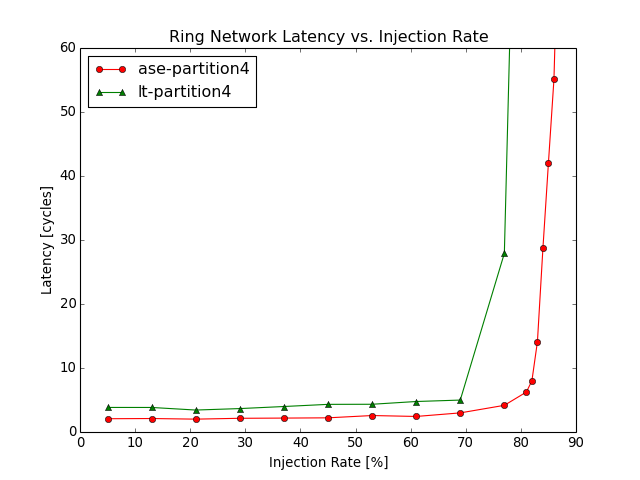
\includegraphics[width=0.33\textwidth]{lab4-net-partition4-plot}
}

\subfigure[Tornado]{
	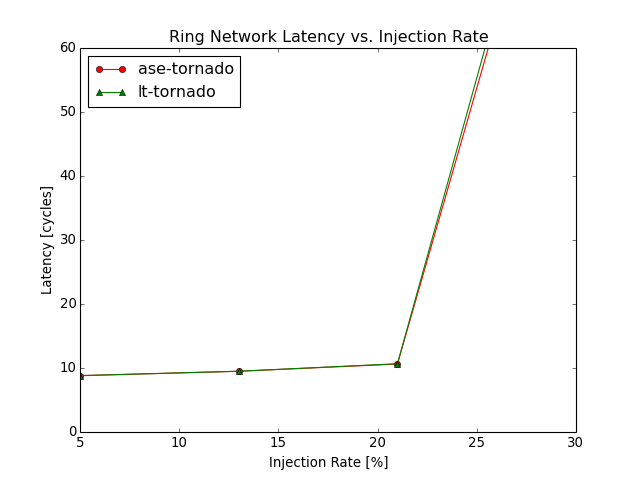
\includegraphics[width=0.33\textwidth]{lab4-net-tornado-plot}
}
\subfigure[Neighbor]{
	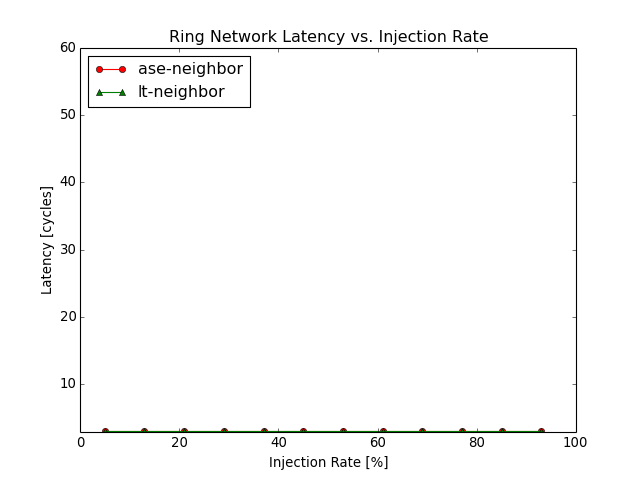
\includegraphics[width=0.33\textwidth]{lab4-net-neighbor-plot}
}
\subfigure[Complement]{
	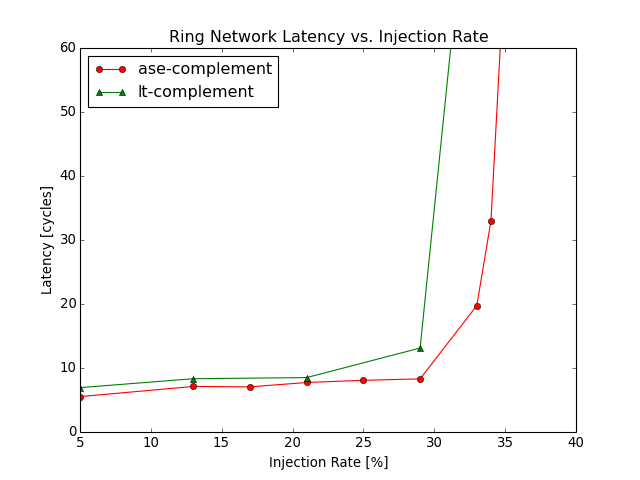
\includegraphics[width=0.33\textwidth]{lab4-net-complement-plot}
}

\subfigure[Reverse]{
	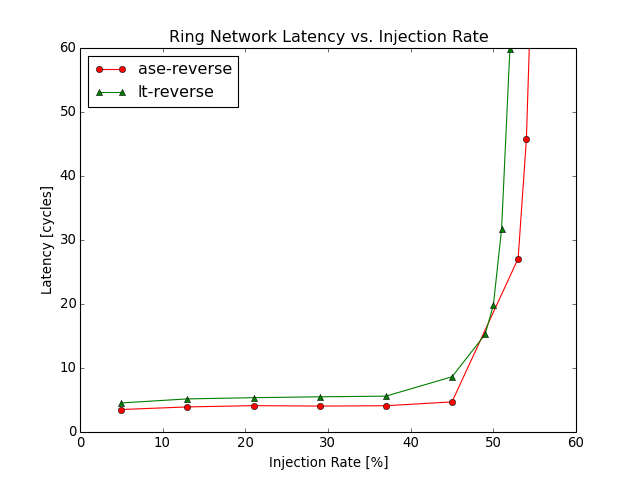
\includegraphics[width=0.33\textwidth]{lab4-net-reverse-plot}
}
\subfigure[Rotation]{
	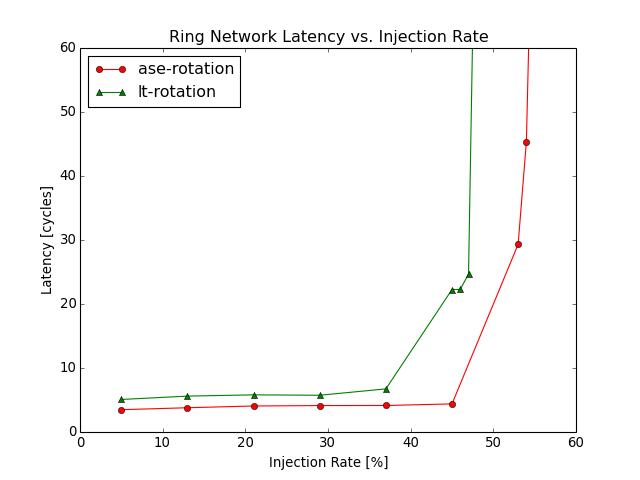
\includegraphics[width=0.33\textwidth]{lab4-net-rotation-plot}
}
\caption{A summary of the behavior of our network under different traffic
		 patterns.}
\label{fig:patterns}
\end{figure}

\end{document}






